\documentclass[conference]{IEEEtran}
\IEEEoverridecommandlockouts
\usepackage{cite}
\usepackage{amsmath,amssymb,amsfonts}
\usepackage{tabularx}
\usepackage{algorithmic}
\usepackage{textcomp}
\usepackage[T1]{fontenc}
\usepackage[utf8]{inputenc}
\usepackage{graphicx}
\usepackage{float}
\usepackage{caption}
\usepackage{subcaption}
\usepackage{booktabs}
\usepackage{array}
\usepackage{multirow}
\usepackage{colortbl}
\usepackage{xcolor}
\usepackage{enumitem}
\usepackage{placeins}
\usepackage{hyperref}
\usepackage{listings}
\usepackage{courier}
% listings style for Python code snippets
\definecolor{codebg}{RGB}{248,248,248}
\definecolor{codeframe}{RGB}{200,200,200}
\definecolor{codecomment}{RGB}{106,153,85}
\definecolor{codestring}{RGB}{206,145,120}
\definecolor{codekw}{RGB}{86,156,214}
\lstdefinestyle{pythonstyle}{
  language=Python,
  backgroundcolor=\color{codebg},
  frame=single,
  rulecolor=\color{codeframe},
  basicstyle=\ttfamily\scriptsize,
  keywordstyle=\color{codekw}\bfseries,
  stringstyle=\color{codestring},
  commentstyle=\color{codecomment}\itshape,
  showstringspaces=false,
  breaklines=true,
  columns=fullflexible,
  keepspaces=true,
  xleftmargin=4pt,
  xrightmargin=4pt,
  aboveskip=4pt,
  belowskip=4pt,
}
\lstset{style=pythonstyle}
% custom column types
\newcolumntype{L}[1]{>{\raggedright\arraybackslash}p{#1}}
\newcolumntype{C}[1]{>{\centering\arraybackslash}p{#1}}
% colors
\definecolor{navy}{RGB}{26,54,93}
\definecolor{steel}{RGB}{46,117,182}
\definecolor{lightblue}{RGB}{219,234,247}
\definecolor{lightgray}{RGB}{245,245,245}
\definecolor{rowgray}{RGB}{235,235,235}
\definecolor{hlgreen}{RGB}{209,231,221}
\definecolor{hlred}{RGB}{248,215,218}
\definecolor{hlyellow}{RGB}{255,243,205}
% macros
\newcommand{\twtp}{T_{\mathrm{WTP}}}   % Worker Tool Predictor time
\newcommand{\twte}{T_{\mathrm{WTE}}}   % Worker Tool Executor time
\def\BibTeX{{\rm B\kern-.05em{\sc i\kern-.025em b}\kern-.08em
    T\kern-.1667em\lower.7ex\hbox{E}\kern-.125emX}}
\begin{document}
\title{SAGE++: Speculative Execution Engine for Agentic Tool Selection%
\thanks{This project is self-funded.}}
\author{\IEEEauthorblockN{Kaveen Jayamanna}
\and
\IEEEauthorblockN{Rabia Usman}}
\maketitle

% ============================================================
\section{Background and Motivation}
% ============================================================
This paper targets a measurable latency bottleneck in the SAGE
framework~\cite{strehlow2026sage}, a benchmarked system for tool-augmented LLM
agents in scalable multi-agent environments.
To address it, we propose SAGE++ (Speculative Augmentation for Generative
Execution), an extension that overlaps the idle period in the Worker's tool
execution cycle with predictive parallel execution, reducing end-to-end latency
without changing SAGE's outputs or safety properties.
Large Language Models have evolved from standalone text generators into the
coordinating cores of agentic pipelines that call APIs, query databases, and
orchestrate specialized sub-agents.
This shift toward tool-augmented LLM agents has produced systems with genuinely
new capabilities, but it has also introduced a class of operational challenges
that sequential transformer inference was never designed to handle.
Among these, \emph{end-to-end response latency} is the most directly user-visible.
The SAGE framework~\cite{strehlow2026sage} evaluates four strategies Simple,
Simple-Tools, Tool-Chain, and Orchestration against a curated benchmark of
102 actions across three Agent Containers (ACs): Smart-Office Services,
Warehouse Management, and Music Player / Playlist Management,
as shown in Table~\ref{tab:sage_results}.

\begin{table}[!h]
\centering
\caption{SAGE benchmark results~\cite{strehlow2026sage}.
  Scores and times: \emph{simple\,/\,complex} queries.
  Orchestration is the bottleneck this project addresses.}
\label{tab:sage_results}
\renewcommand{\arraystretch}{1.3}
\resizebox{\columnwidth}{!}{%
\begin{tabular}{l c c c}
\toprule
\rowcolor{navy}
\color{white}\textbf{Method}
  & \color{white}\textbf{Score (1--5)}
  & \color{white}\textbf{Time (s)}
  & \color{white}\textbf{Tokens (M)} \\
\midrule
Simple        & 4.52\,/\,3.81 & 2.36\,/\,6.14   & 3.478 \\
\rowcolor{rowgray}
Simple-Tools  & 4.68\,/\,4.20 & 5.24\,/\,8.45   & 3.120 \\
Tool-Chain    & 4.72\,/\,4.00 & 6.81\,/\,9.99   & 3.036 \\
\rowcolor{hlred}
Orchestration & 4.16\,/\,3.71 & \textbf{14.26\,/\,16.98} & \textbf{2.557} \\
\bottomrule
\end{tabular}}
\end{table}

Orchestration achieves its low token count through a divide-and-conquer
decomposition: the Orchestrator exposes only agent names, not full action
descriptions, to each sub-planner, sharply reducing input tokens per LLM call.
The tradeoff is a minimum of six sequential LLM invocations per request
(Orchestrator, Planner LLM, Tool Predictor Worker, Tool Execution Worker,
Evaluator, Overall Evaluator, Output Generator), each blocked on the previous
step's output.
That chain is the structural source of the latency problem.
Independent empirical evidence is provided by~\cite{drammeh2025multiagent}, who
evaluated single-agent and multi-agent LLM architectures across 348 controlled
trials.
Both configurations converge to roughly 40\,s end-to-end latency, suggesting
that orchestration does not yield meaningful speed improvements.
The primary benefit of multi-agent systems is improved decision quality and
reliability, not reduced response time.
The latency overhead introduced by orchestration appears systematic, persistent,
and only partially mitigable through architectural optimisation.

% ============================================================
\section{Objective}
% ============================================================
The objective of SAGE++ is to reduce the end-to-end response latency of the
SAGE Orchestration method by eliminating the idle period in the Worker Tool
Predictor to Worker Tool Executor handoff within each Agent-Trio, without
degrading response quality, token efficiency, or safety.
SAGE++ introduces a speculative shadow thread that predicts and executes the
most likely tool call(s) \emph{in parallel} with the Worker Tool Predictor's
reasoning.
On a correct prediction (a ``hit''), the Worker Tool Executor's result is
already available the moment the Worker Tool Predictor finishes, reducing the
effective cycle time to:
\begin{equation}
T_{\mathrm{total}} = \max\!\bigl(\twtp,\; \twte\bigr)
\label{eq:overlapped}
\end{equation}
where $\twtp$ is the Worker Tool Predictor generation time and $\twte$ is the
Worker Tool Executor dispatch-to-result time.
On a miss, the speculative result is discarded and the system falls back to
baseline behaviour with no extra cost.
Worst-case latency under SAGE++ is identical to the unmodified SAGE
Orchestration method.

\section{Status of Research}
\subsection{Speculation and Parallelism in Agent Systems}
Ye et al.~\cite{ye2025speculative} introduced Speculative Actions, the closest
conceptual predecessor to our work.
Their Speculator--Actor framework runs a fast model in parallel to predict the
next agent action while the primary Actor executes, achieving up to 50\%
theoretical latency reduction under simple assumptions, with empirical
wall-clock savings verified across four environments including ALFWorld and
WebArena.
Speculative Actions targets general multi-step sequential action prediction
rather than the bounded idle window that exists between the Worker Tool
Predictor and Worker Tool Executor inside a SAGE Agent-Trio.
Huang et al.~\cite{huang2025spagent} present SPAgent, an algorithm-system
co-design that introduces a two-phase adaptive speculation mechanism and a
two-level scheduler to regulate speculative requests under varying engine load.
SPAgent achieves up to $1.65\times$ end-to-end speedup on LLM search agents
while maintaining or improving accuracy.
Although SPAgent demonstrates the viability of speculation in multi-step search
settings, its design targets general reasoning-tool interaction rather than the
strictly delineated Worker Tool Predictor -- Worker Tool Executor -- Evaluator
architecture of SAGE Agent-Trios.
Gim et al.~\cite{gim2024asynclm} propose AsyncLM, which overlaps LLM inference
with function-call execution through an interrupt-based notification protocol.
AsyncLM achieves end-to-end latency reductions of $1.6\times$--$5.4\times$ on
BFCL benchmark tasks.
It operates within a single LLM's function-call context and does not classify
tools by their side-effect profile before speculation.
Guan et al.~\cite{guan2025dsp} introduce Dynamic Speculative Planning (DSP), an
asynchronous online reinforcement learning framework that jointly optimises
end-to-end latency and inference cost without requiring additional pre-deployment
training.
DSP achieves comparable efficiency to the fastest existing lossless acceleration
methods while reducing total cost by 30\% and unnecessary computation by up to
60\%.
Its RL-based adaptive routing differs fundamentally from the structured Worker
Tool Predictor handoff in SAGE, and it does not provide deterministic safety
guarantees for speculative execution.

\subsection{Planning Optimisation and Parallel Execution}
Zhang et al.~\cite{zhang2025apc} propose Agentic Plan Caching (APC), which
extracts structured plan templates at test-time and reuses them for semantically
similar queries.
APC reduces latency by 27.28\% and cost by 50.31\% on average while maintaining
response quality.
APC and SAGE++ are complementary strategies: APC avoids the planning step
entirely on cache-hit queries, while SAGE++ accelerates execution within any
Agent-Trio cycle irrespective of whether a cached plan was available.
Xiao et al.~\cite{xiao2025m1parallel} achieve approximately $3\times$ speedups
through M1-Parallel by launching multiple agent instances in parallel and
committing the fastest result.
The approach is computationally expensive, as resources are spent on all
non-winning threads, which are discarded, and there is no guarantee of bounded
overhead on incorrect paths.
Saha et al.~\cite{saha2025system1x} apply dual-process cognitive theory to LLM
planning, training a controller to choose between fast (System-1) and deliberate
(System-2) reasoning depending on query difficulty.
The work is conceptually related to our Hazard Detection Unit's classification
logic, but it addresses reasoning-path selection rather than tool-execution
parallelism.

\subsection{Token-Level Speculative Decoding}
Leviathan et al.~\cite{leviathan2023speculative} introduce speculative decoding,
the conceptual ancestor of our approach: a draft model proposes multiple tokens
in parallel, which a larger model verifies in one forward pass, achieving
$2\times$--$3\times$ acceleration on T5-XXL without changing output distributions.
Cai et al.~\cite{cai2024medusa} extend this with multiple decoding heads attached
to the base model.
Zhang et al.~\cite{zhang2025swiftspec} scale asynchronous speculative decoding
further for ultra-low-latency LLM inference.
We borrow the commit-or-rollback contract from this family of work and apply it
at the inter-module coordination level, targeting the handoff boundary between
two distinct Worker modules rather than token generation within a single model.

\subsection{Identified Gaps}
\label{sec:gaps}
The survey above surfaces four specific gaps that no existing system closes
simultaneously.
\begin{enumerate}
\item \textbf{The Worker Tool Executor handoff is unaddressed.}
Existing speculation work targets general multi-step action sequences
\cite{ye2025speculative, guan2025dsp}, single-LLM function-call concurrency
\cite{gim2024asynclm}, or token-level generation
\cite{leviathan2023speculative, cai2024medusa}.
None exploits the specific bounded idle window during which the Worker Tool
Executor waits for the Worker Tool Predictor inside an Agent-Trio.
\item \textbf{No principled safety classification for speculative execution.}
AsyncLM and Speculative Actions introduce parallelism, but neither classifies
tools by their side-effect profile before executing speculatively.
For systems managing persistent state, warehouse write operations, customer
record mutations, speculatively executing a state-changing tool and then
rolling back on a misprediction may be irreversible.
No prior architecture provides a deterministic Safe/Unsafe classification gate.
\item \textbf{Predictor granularity is unstudied for tool selection.}
No prior system compares frequency-cache, classical ML, and small-LLM predictor
designs specifically for the tool-selection task within a unified benchmark,
making it impossible to determine the accuracy-overhead tradeoff for this workload.
\item \textbf{Weak misprediction cost guarantees.}
M1-Parallel wastes resources on discarded threads~\cite{xiao2025m1parallel}.
Adaptive routing frameworks~\cite{saha2025system1x, guan2025dsp} do not bound
worst-case overhead on misprediction.
No prior architecture formally guarantees that a miss costs no more than the
unmodified baseline.
\end{enumerate}

% ============================================================
\section{Problem Statement}
% ============================================================
The SAGE Orchestration method achieves superior modularity and token efficiency
but takes 14.26\,s (simple) and 16.98\,s (complex) per request, roughly
2--7$\times$ slower than simpler alternatives~\cite{strehlow2026sage}.
The structural cause is a hard sequential dependency inside each Agent-Trio.
When the Orchestrator assigns a subtask to an Agent-Trio, execution proceeds
in strict order:
\begin{enumerate}[itemsep=2pt]
  \item The \textbf{Worker Tool Predictor} receives the subtask, reasons over
        all available tools across the three ACs, and outputs a tool selection.
  \item The \textbf{Worker Tool Executor} receives that output and translates it
        into concrete, schema-valid API calls against the OPACA platform but is
        \emph{completely blocked} and idle until Step~1 finishes.
  \item The \textbf{Evaluator} verifies the tool results against the original
        subtask specification.
\end{enumerate}
During Step~1, the Worker Tool Executor is completely idle.
There is no logical requirement for this: the Worker Tool Executor does not need
the Worker Tool Predictor's complete output, only an accurate prediction of what
that output will be.
On workloads where the same tool is invoked repeatedly, or where request
semantics strongly constrain the likely tool choice, this prediction is
achievable with a lightweight model.
Figure~\ref{fig:arch_sequential} illustrates the current blocking architecture.

\begin{figure}[!htbp]
  \centering
  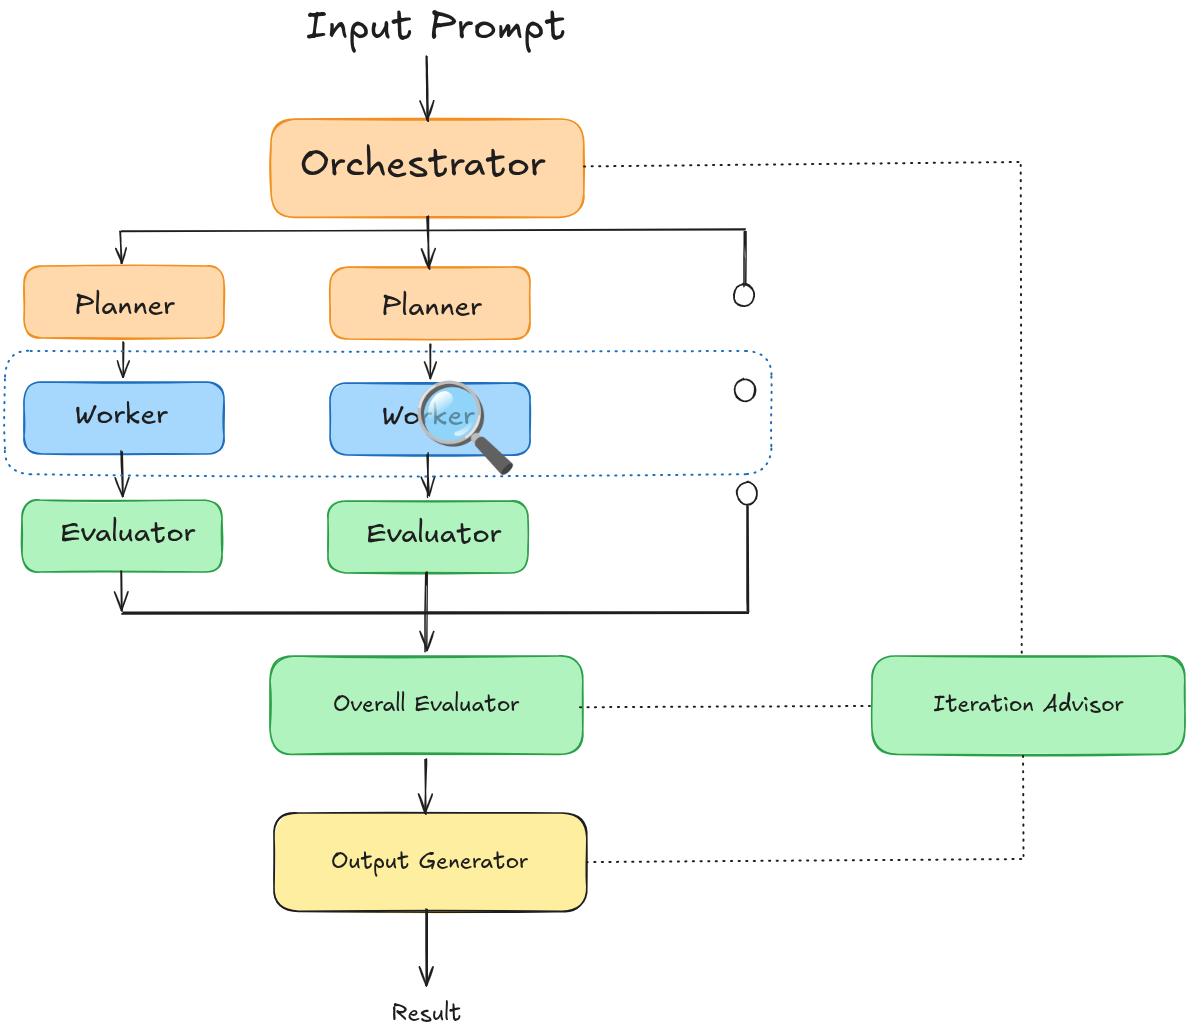
\includegraphics[width=\linewidth]{figures/fig_arch_sequential.png}
  \caption{SAGE Agent-Trio sequential architecture.
    The Worker Tool Executor is blocked and idle throughout the entire
    Worker Tool Predictor phase, accumulating avoidable latency equal
    to $\twtp$. SAGE++ is an incremental improvement to the worker component highlighted in blue.}
  \label{fig:arch_sequential}
\end{figure}

\subsection{Practical Constraints}
Any solution must satisfy four non-negotiable constraints:
\begin{enumerate}[itemsep=3pt]
  \item \textbf{Quality preservation.} Response quality scores must remain
        statistically equivalent to the SAGE Orchestration baseline.
  \item \textbf{Safety.} State-changing tool calls must never execute
        speculatively. Incorrect speculative writes cannot be reliably rolled
        back in the Warehouse AC.
  \item \textbf{Zero misprediction overhead.} A failed prediction must incur no
        additional latency beyond the unmodified baseline.
  \item \textbf{Low predictor overhead.} The prediction mechanism must be fast
        enough that its own inference cost does not negate the savings it enables.
\end{enumerate}

% ============================================================
\section{Design}
% ============================================================
\subsection{Architectural Overview}
SAGE++ replaces the idle gap between the Worker Tool Predictor and the Worker
Tool Executor with a speculative shadow thread.
The moment a subtask arrives at an Agent-Trio, two threads activate simultaneously:
\begin{itemize}[itemsep=3pt]
  \item \textbf{Main Thread:} The Worker Tool Predictor begins its normal
        reasoning process, unchanged from the original SAGE design.
  \item \textbf{Shadow Thread:} A lightweight Predictor immediately guesses the
        most likely tool call.
        The Hazard Detection Unit checks whether this tool is classified as Safe.
        If so, the Speculative Execution Engine dispatches the call immediately.
\end{itemize}
When the Worker Tool Predictor completes, the Commit/Flush Logic compares its
decision against the Reorder Buffer's pending result:
\begin{itemize}[itemsep=3pt]
  \item \textbf{Hit:} The speculative result is committed. The Worker Tool
        Executor skips execution entirely.
        Effective cycle time $= \max(\twtp,\, \twte)$.
  \item \textbf{Miss:} The Reorder Buffer is flushed, the shadow thread is
        discarded, and the correct tool is dispatched through the normal Worker
        Tool Executor path.
        Effective cycle time $= \twtp + \twte$, identical to baseline.
\end{itemize}
Figure~\ref{fig:arch_speculative} shows the full SAGE++ architecture.

\begin{figure}[!htbp]
  \centering
  \includegraphics[width=\linewidth]{figures/fig_arch_speculative_refined.png}
  \caption{SAGE++ Speculative Threading Architecture.
    Orange boxes are existing SAGE components (Main Thread).
    Blue boxes are the four new SAGE++ components (Speculative Thread):
    Predictor, Hazard Detection Unit, Speculative Execution Engine,
    and Reorder Buffer.
    Dashed arrows show the commit/flush decision at the Worker Tool Predictor
    boundary.}
  \label{fig:arch_speculative}
\end{figure}

\subsection{Component Details}
\subsubsection{Predictor (Branch Prediction Unit)}
The Predictor fires the moment a subtask arrives, before the Worker Tool
Predictor has produced a single token.
We implement and compare three variants of increasing semantic power:
\begin{itemize}[itemsep=3pt]
  \item \textbf{Habit-Based Predictor.}
        An LRU frequency cache mapping subtask signatures to historically
        most-common tool selections.
        Overhead: $\mathcal{O}(1)$ lookup.
        Works best when the same tools get called repeatedly across the three ACs.
  \item \textbf{Classical ML Predictor.}
        A Na\"{i}ve Bayes classifier trained on TF-IDF keyword features extracted
        from past subtask text.
        More generalizable than a frequency cache while remaining sub-millisecond
        at inference time.
  \item \textbf{Small LLM Predictor.}
        A distilled transformer (DistilBERT-base or Phi-family) providing
        lightweight semantic understanding of the full subtask context.
        Highest accuracy at the cost of a small additional inference step.
\end{itemize}
The accuracy-overhead tradeoff across these three variants is one of the primary
empirical questions this project investigates.

\subsubsection{Hazard Detection Unit}
Classifies every tool in the SAGE environment at system initialisation:
\begin{itemize}[itemsep=3pt]
  \item \textbf{Safe (Idempotent):} Read-only operations---sensor queries
        (Smart-Office AC), playlist reads (Music Player AC), meeting-room lookups.
        Discarding a speculative result has no side effects.
  \item \textbf{Unsafe (State-Changing):} Write operations, deletions, order
        placements, warehouse inventory updates, customer record modifications
        (Warehouse AC). Speculative execution is blocked unconditionally.
\end{itemize}
This classification is computed once at startup and adds zero runtime overhead
per request.

\subsubsection{Speculative Execution Engine}
The Engine manages the shadow thread's lifecycle: it receives the Predictor's
output, verifies the Hazard Detection Unit's classification, and launches the
tool call in a dedicated thread via the standard OPACA interface.
It handles thread lifecycle, timeout management, and result hand-off to the
Reorder Buffer.

\subsubsection{Reorder Buffer (ROB)}
The ROB holds the speculative result in a pending state.
On a hit, it promotes the result to committed status and forwards it to the
Evaluator immediately.
On a miss, it flushes in $\mathcal{O}(1)$ time and signals the Worker Tool
Executor to dispatch the correct call through the standard path.
The flush adds no latency overhead beyond what the original system would have
incurred.

\subsection{Contribution}
Three properties together distinguish SAGE++ from all prior work:
\begin{enumerate}[itemsep=3pt]
  \item \textbf{First application to the Worker Tool Executor handoff.}
        We identify the specific bounded idle window during Worker Tool Predictor
        reasoning as a distinct and previously unexploited bottleneck class in
        orchestrated agent architectures.
  \item \textbf{Deterministic safety via hazard classification.}
        The Hazard Detection Unit provides a binary Safe/Unsafe label before any
        speculation occurs, preventing state-corrupting execution without runtime
        cost.
  \item \textbf{Formal zero-overhead misprediction guarantee.}
        The Reorder Buffer flush ensures the miss path is identical to baseline
        latency, a bound that no prior speculative agent system provides.
\end{enumerate}

% ============================================================
\section{Methodology}
% ============================================================
\subsection{Dataset}
We use the SAGE benchmark containers from~\cite{strehlow2026sage}, consisting
of 180 simple and 39 complex query prompts executed against three Agent
Containers (ACs):
\begin{itemize}[itemsep=3pt]
  \item \textbf{Smart-Office Services.} Meeting scheduling, room booking, and
        sensor queries. Predominantly read-heavy; the majority of actions are
        classified as Safe.
  \item \textbf{Warehouse Management.} Order creation, stock updates, and
        customer record operations.
        Contains most of the Unsafe (state-changing) actions; this domain is
        the primary test of the Hazard Detection Unit.
  \item \textbf{Music Player / Playlist Management.} Playback controls, playlist
        reads, and playlist writes. Mixed Safe/Unsafe profile.
\end{itemize}
In total, 15 agents expose 102 actions.
Each benchmark prompt is annotated with an expected answer and expected tool
calls, supporting both LLM-judge quality scoring (1--5) and exact tool-match
evaluation.

\subsection{Implementation}
SAGE++ is implemented as a \texttt{SpeculativeAgentTrio} Python subclass that
extends SAGE's existing \texttt{AgentTrio} without modifying any original module.
Switching between the original SAGE and SAGE++ requires only changing a single
configuration flag in the benchmark runner.
The predictor component is an abstract class realized by four concrete variants
described below.

\begin{description}[leftmargin=0pt, itemsep=3pt, topsep=4pt]
  \item[\textbf{Hazard Detection Unit.}]
  All 102 benchmark actions were manually reviewed and classified as Safe or
  Unsafe, stored in a static lookup table loaded at agent startup.
  A runtime enforcement gate intercepts every speculative dispatch and blocks
  any Unsafe tool before it reaches the OPACA platform.

  \item[\textbf{Speculative Execution Engine.}]
  Spawns a shadow thread in parallel with the Worker Tool Predictor.
  Receives the Predictor output, checks the Hazard label, and if Safe, dispatches
  the tool call via the standard OPACA interface.
  A configurable timeout prevents a slow speculative call from blocking the
  commit decision.

  \item[\textbf{Reorder Buffer.}]
  When the Worker Tool Predictor completes, the Commit/Flush Logic compares its
  tool selection against the ROB's pending entry.
  On a hit, the result is forwarded directly to the Evaluator, bypassing the
  Worker Tool Executor entirely.
  On a miss the ROB flushes and normal execution continues.

  \item[\textbf{Habit-Based Predictor.}]
  A recency-oriented lightweight memory model rather than a semantic or
  supervised classifier.
  Each prompt is reduced to a compact signature via first-line tokenization,
  identifier normalization, lowercasing, and numeric removal; the signature is
  then mapped to the most recently observed tool-call sequence for that pattern,
  as illustrated below:
\begin{lstlisting}
cache["what is the device health"] = [
    ("GetDeviceId",       {"device_name": "router"}),
    ("CheckDeviceHealth", {"device_id": 3}),]
\end{lstlisting}
  When an exact match fails the predictor falls back to the most recently used
  sequence within the compatible tool family, allowing it to reuse patterns even
  when prompt wording varies.
  The predictor is evaluated as an online cache over the full 219-prompt
  benchmark stream starting from an empty state.
  A sweep over working-set sizes $k \in \{1, 2, \ldots, 200\}$ identifies
  $k{=}1$ as optimal, achieving \textbf{40.6\%} overall full tool-sequence
  accuracy (48.6\% on simple queries, 5.0\% on complex), as shown in
  Figure~\ref{fig:habit_sweep}.

  \begin{figure}[!htbp]
    \centering
    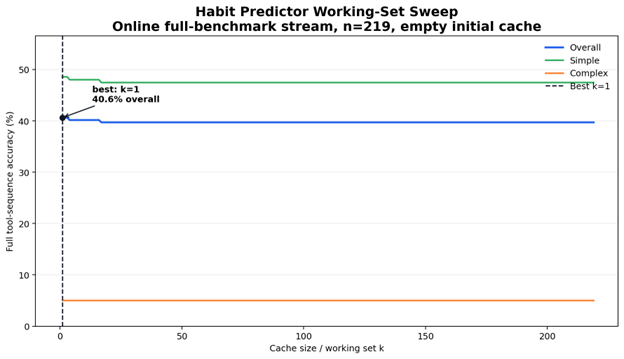
\includegraphics[width=\linewidth]{figures/fig_habit_sweep.png}
    \caption{Habit predictor working-set sweep over the full 219-prompt online
      benchmark stream.
      Accuracy peaks at $k{=}1$ (40.6\% overall), with simple-query performance
      (48.6\%) far exceeding complex-query performance (5.0\%).
      The flat curve confirms that larger caches add no benefit.}
    \label{fig:habit_sweep}
  \end{figure}

  This locality-based behavior proves particularly beneficial on simple queries,
  where prompts cluster around related tasks such as availability checks or
  room-name lookups: a second room-name request may carry a unique signature but
  still require the same tool type as the first, which the predictor handles via
  the compatible-tool fallback.
  On complex queries---where sequences are longer and repetition is rare---accuracy
  falls to 5.0\%, reflecting the limits of short-range ordering locality rather
  than any semantic understanding.

  \item[\textbf{Na\"{i}ve Bayes Predictor.}]
  A Multinomial Na\"{i}ve Bayes classifier that learns a direct probabilistic
  mapping from natural-language prompt features to tool-call sequences.
  The training corpus consists of 131 benchmark prompts augmented with synthetic
  label-style demonstrations (e.g., ``Get Room Name'' mapped to its corresponding
  function call), yielding a final training set of 509 rows.
  The training process establishes conditional probabilities of tool sequences
  given observed lexical features:
\begin{lstlisting}
train_example = (
    "What is the name of room 3?",
    [("GetRoomName", {"room_id": 3})],
)
\end{lstlisting}
  During inference the predictor evaluates a new prompt against the learned
  distribution to determine the most probable tool-call sequence:
\begin{lstlisting}
prompt     = "Tell me the name of room 3"
prediction = [("GetRoomName", {"room_id": 3})]
\end{lstlisting}
  Candidate predictions are strictly constrained to the active tool family of
  the current Worker Agent, and the output is returned as a structured
  \texttt{ToolPrediction} object.
  Training-split accuracy is \textbf{95.4\%} overall (98.9\% simple,
  86.5\% complex); generalization is assessed against an 88-prompt held-out set
  that is shared with the few-shot SmallLLM evaluation.

  \item[\textbf{Small LLM Predictor--Zero-Shot.}]
  Uses \texttt{typeform/distilbert-base-uncased-mnli}
  (DistilBERT, ${\approx}$66M parameters) as a zero-shot NLI backbone.
  The user prompt and the suite of candidate tool descriptions are passed
  together; the model scores each tool via natural language inference and selects
  the highest-scoring option, requiring no task-specific training demonstrations:
\begin{lstlisting}
prompt          = "What is the current volume in the meeting room?"
candidate_tools = ["GetRoomId", "GetCurrentVolume", "SetCurrentVolume"]
prediction      = [
    ("GetRoomId",         {"room_name": "meeting room"}),
    ("GetCurrentVolume",  {"room_id": 2}),
]
\end{lstlisting}

  \item[\textbf{Small LLM Predictor--Few-Shot.}]
  The same DistilBERT architecture augmented with concrete prompt-label pairs
  drawn from the 131-prompt training split as contextual demonstrations.
  Historical examples guide the mapping of new requests to their respective
  action sequences, providing a more robust performance profile than the zero-shot
  variant on queries that closely resemble seen examples:
\begin{lstlisting}
train_examples = [
    (
        "What is the current volume in the meeting room?",
        [("GetRoomId",        {"room_name": "meeting room"}),
         ("GetCurrentVolume", {"room_id": 2})],
    ),
    (
        "Lower the volume in the office to 20%",
        [("GetRoomId",           {"room_name": "office"}),
         ("SetCurrentVolume",    {"room_id": 1, "volume": 20})],
    ),
]
prompt     = "Check the current volume in the office"
prediction = [
    ("GetRoomId",        {"room_name": "office"}),
    ("GetCurrentVolume", {"room_id": 1}),
]
\end{lstlisting}
\end{description}

\subsection{Evaluation Metrics}
\label{sec:metrics}
\begin{table}[H]
\centering
\caption{Evaluation metrics and success criteria.}
\label{tab:metrics}
\renewcommand{\arraystretch}{1.3}
\begin{tabularx}{\columnwidth}{p{1.9cm} X X}
\toprule
\rowcolor{navy}
\color{white}\textbf{Metric} &
\color{white}\textbf{Definition} &
\color{white}\textbf{Success Criterion} \\
\midrule
End-to-end latency
& Total response time (s) per request on the benchmark dataset
& Statistically significant reduction vs.\ SAGE baseline \\
\rowcolor{rowgray}
Predictor hit rate
& Fraction of speculative calls where predicted tool matches Worker Tool
  Predictor decision
& Compare all three predictor types; report by simple and complex split \\
Safety audit
& Count of Unsafe tools executed speculatively during benchmark run
& \textbf{Zero violations.} Any violation invalidates the safety guarantee \\
\rowcolor{rowgray}
Response quality
& Judge-LLM score (1--5) on final answers
& No statistically significant regression vs.\ SAGE baseline \\
Miss overhead
& Extra latency on a misprediction path vs.\ baseline
& $\Delta t \leq 5\%$ of baseline; flush must be ${\approx}0$ \\
\bottomrule
\end{tabularx}
\end{table}

% ============================================================
\section{Hypotheses}
% ============================================================
\begin{description}[leftmargin=0pt, itemsep=6pt]
\item[\textbf{H1--Latency Reduction.}]
Incorporating the speculative execution engine into the SAGE Worker Agent
reduces total query processing time by up to 2.5\% for simple queries and up
to 3.2\% for complex queries.
At high predictor accuracy the effective cycle time approaches
$\max(\twtp,\, \twte)$.
\item[\textbf{H2--Predictor Tradeoff.}]
The Small LLM Predictor achieves higher hit rates than the Habit-Based and
Na\"{i}ve Bayes predictors on diverse query distributions.
On repetitive or domain-constrained workloads across the three ACs where the
LRU cache saturates early, this advantage narrows, and a crossover exists where
the Small LLM's inference overhead negates its accuracy advantage.
\item[\textbf{H3--Safety Soundness.}]
The Hazard Detection Unit correctly classifies all 102 benchmark actions at
initialization, and no Unsafe tool is executed speculatively at any point
during benchmark evaluation across all three ACs.
\end{description}

% ============================================================
\section{Challenges}
% ============================================================

\subsection{Challenge I: Python GIL and True Parallelism}
The first challenge in implementing SAGE++ is the restriction imposed by the
traditional Global Interpreter Lock (GIL) in CPython, illustrated in
Figure~\ref{fig:gil}.
Even though both the main \texttt{asyncio} event loop and the shadow thread can
be scheduled concurrently, the CPython runtime permits only one thread to execute
Python bytecodes at a time.
As a result, CPU-bound portions of speculation which are prediction, hazard checking, and ROB management, they continue to compete with the main WorkerAgent execution
thread, reducing the effective overlap between the two paths.

\begin{figure}[!htbp]
  \centering
  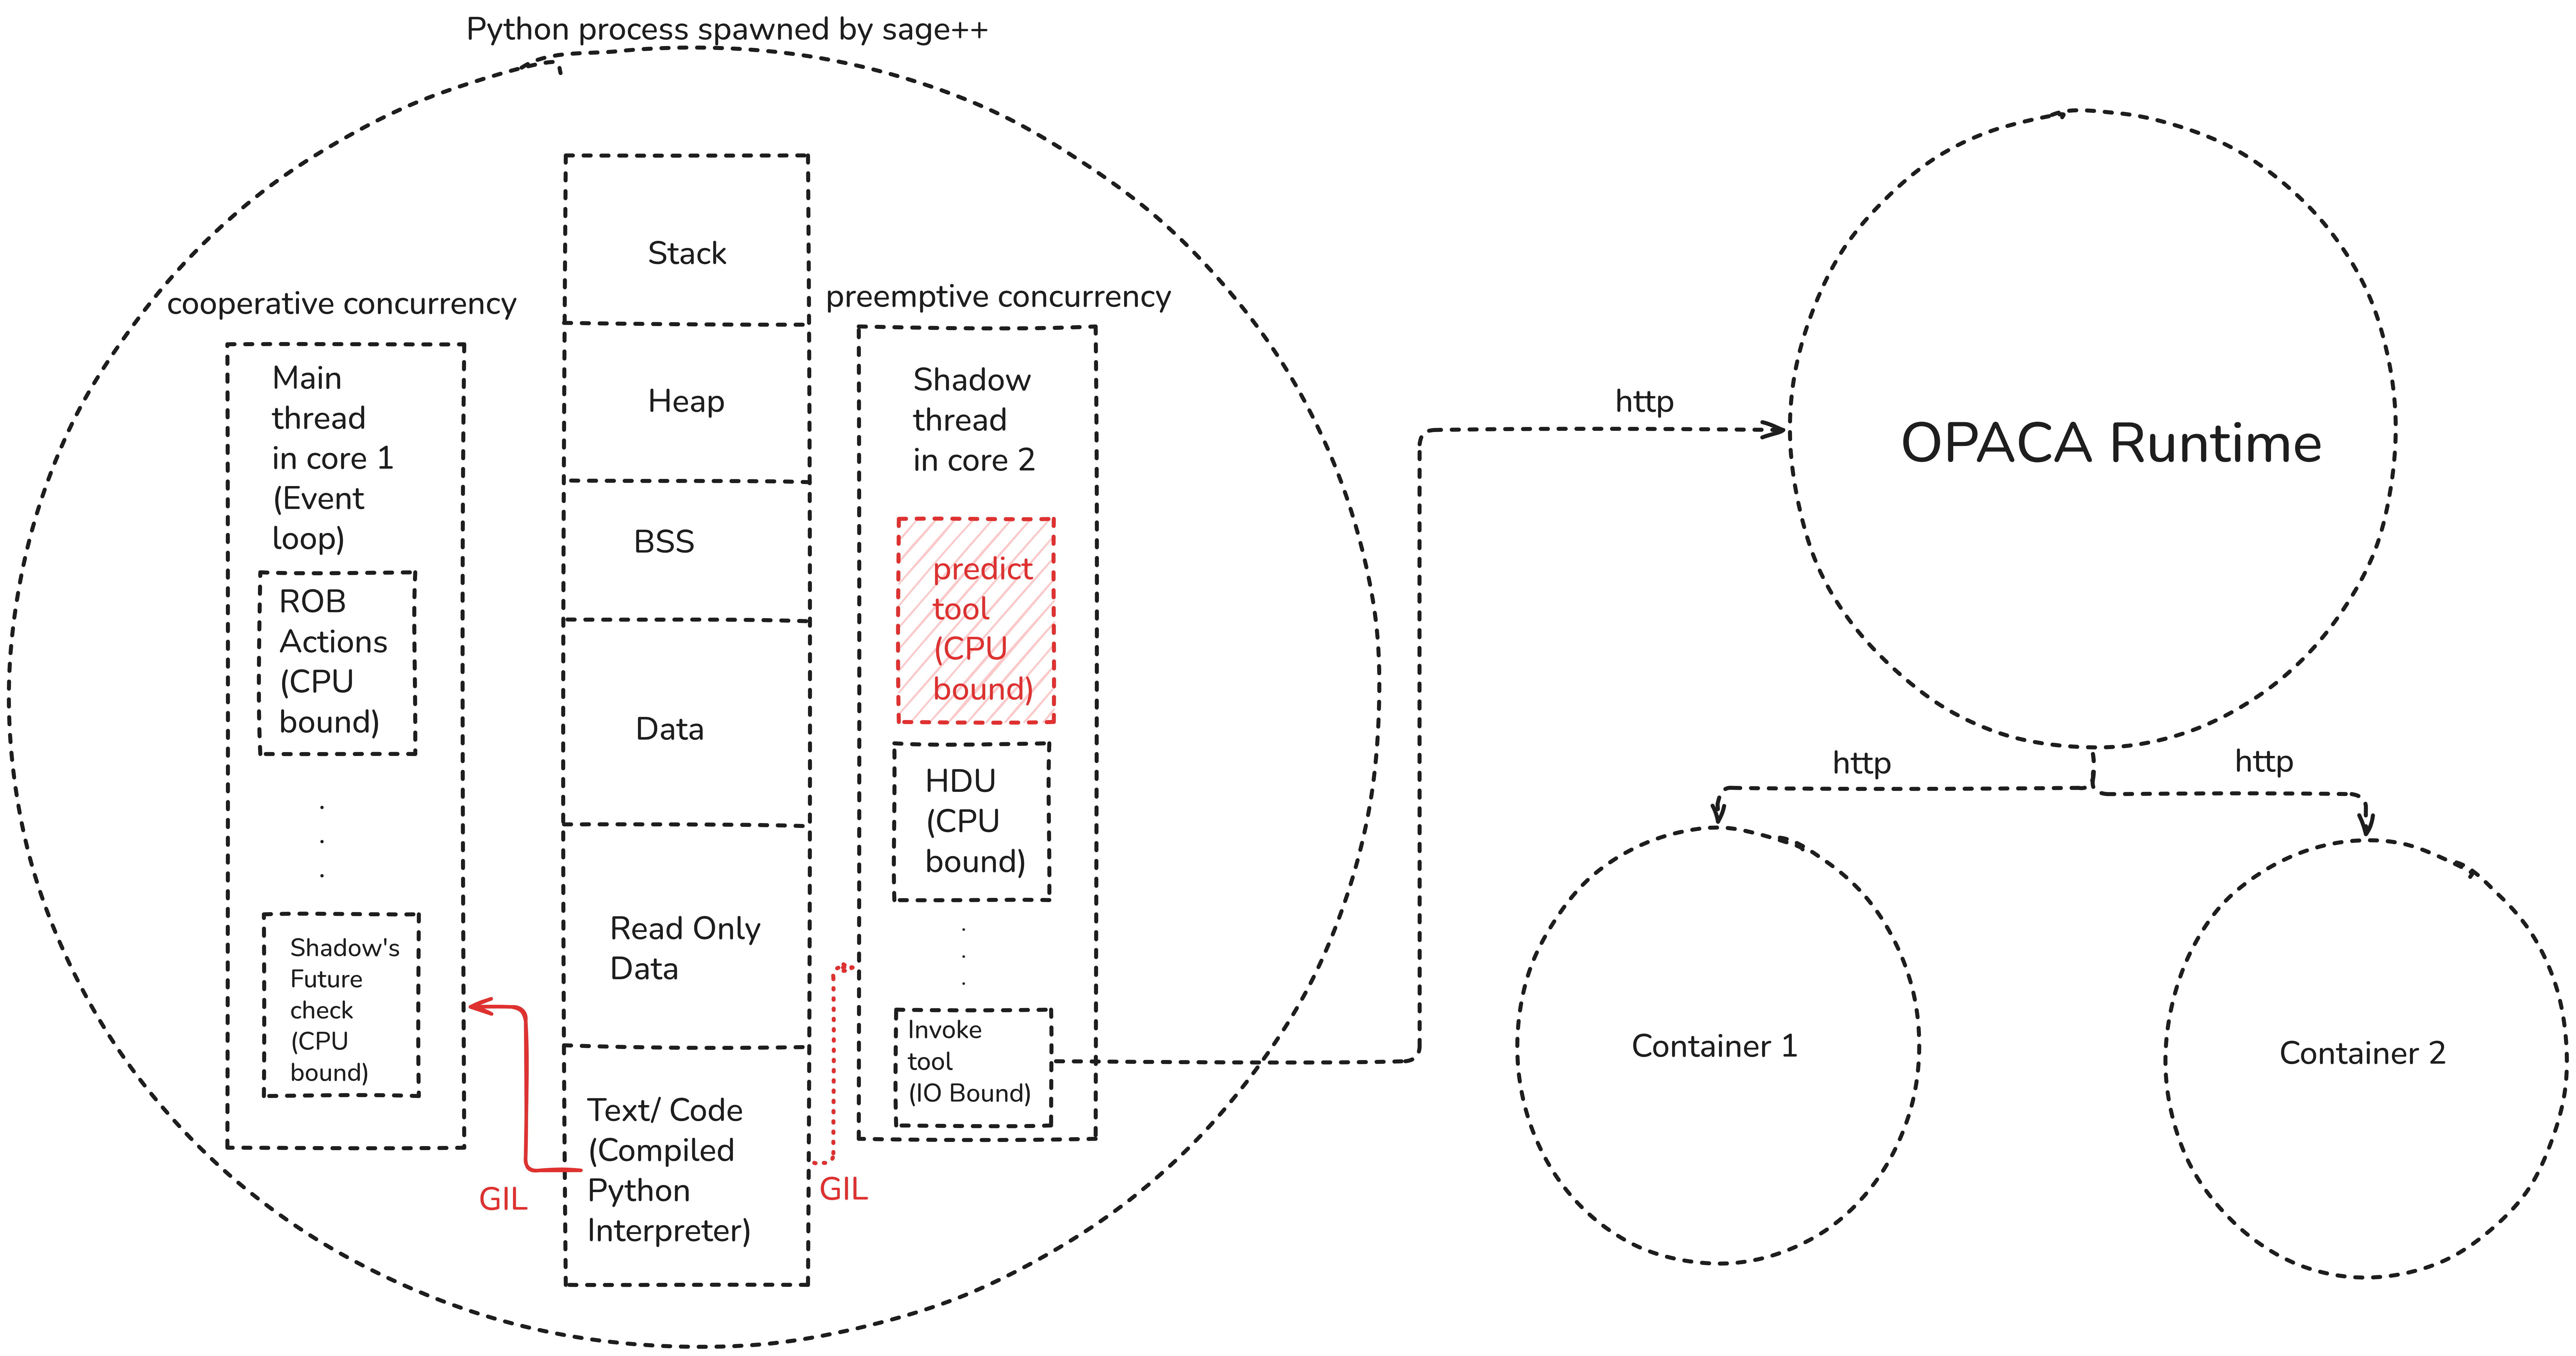
\includegraphics[width=\linewidth]{figures/fig_gil_architecture.png}
  \caption{Python process architecture for SAGE++.
    The main thread (core~1, cooperative concurrency via \texttt{asyncio}) and
    shadow thread (core~2, preemptive concurrency) share heap and data segments.
    Under the standard GIL only one thread executes Python bytecodes at a time;
    free-threaded CPython~3.14 removes this constraint, enabling true parallel
    execution of prediction (CPU-bound) and tool invocation (I/O-bound).}
  \label{fig:gil}
\end{figure}

We address this by switching to the free-threaded CPython~3.14 build, which
removes the GIL and permits multiple Python threads to run in parallel on
separate cores~\cite{python314freethreading}.
The main event loop retains responsibility for controlling speculation and
committing results; the shadow thread independently runs prediction, hazard
checking, and speculative OPACA calls.
Thread safety is enforced through synchronization primitives in the Reorder
Buffer, so the speculative execution algorithm itself requires no modification.

\subsection{Challenge II: Correctness Under Parallelism}
Introducing a speculative thread alongside the main orchestration path creates
three distinct correctness risks: race conditions on the Reorder Buffer, unsafe
side effects from premature speculation, and performance degradation from
incorrect predictions.

To address \textbf{race conditions}, all ROB operations (\texttt{store()},
\texttt{commit()}, and \texttt{flush()}) are protected by a
\texttt{threading.Lock}, ensuring that the main thread sees only a fully committed result or nothing at all, never a partially written intermediate state.

To prevent \textbf{unsafe side effects}, the Hazard Detection Unit
unconditionally blocks any non-read or write-like action from entering the
speculative path.
No state mutation reaches the OPACA platform until the WorkerAgent has committed
to the tool selection.

When a prediction is \textbf{incorrect} whether in the tool name or its arguments, a cancellation event is triggered, the ROB is flushed, and the speculative result is discarded.
In this scenario SAGE++ degrades gracefully to standard SAGE orchestration
behavior with no added overhead.

\subsection{Challenge III: Asyncio-Thread Coordination}
The third challenge is coordinating the primary \texttt{asyncio} event loop and the shadow thread without accidentally serializing the two paths or introducing deadlocks.
If the main thread blocks waiting for the shadow thread to finish, the optimization collapses to sequential execution, if no synchronization exists, the main thread may compare tool selections against an inconsistent ROB state.

SAGE++ resolves this with a lightweight \texttt{prediction\_future} object,
shown in Figure~\ref{fig:coordination}.
When a new subtask arrives the main event loop (i)~launches the shadow thread
and (ii)~immediately issues the standard LLM call for the WorkerAgent.
The shadow thread first runs \texttt{predict()}, then signals the main path via
\texttt{loop.call\_soon\_threadsafe()}.
Both expensive operations then proceed concurrently:
\texttt{asyncio.gather(prediction\_future, call\_llm())} awaits both on separate
cores while the shadow thread issues the speculative HTTP request to OPACA.
After both resolve, the main path compares the predicted and actual tool
selections: a match commits the ROB result; a mismatch sets
\texttt{cancel\_event}, flushes the ROB, and invokes the correct tool through
the standard path.

\begin{figure}[!htbp]
  \centering
  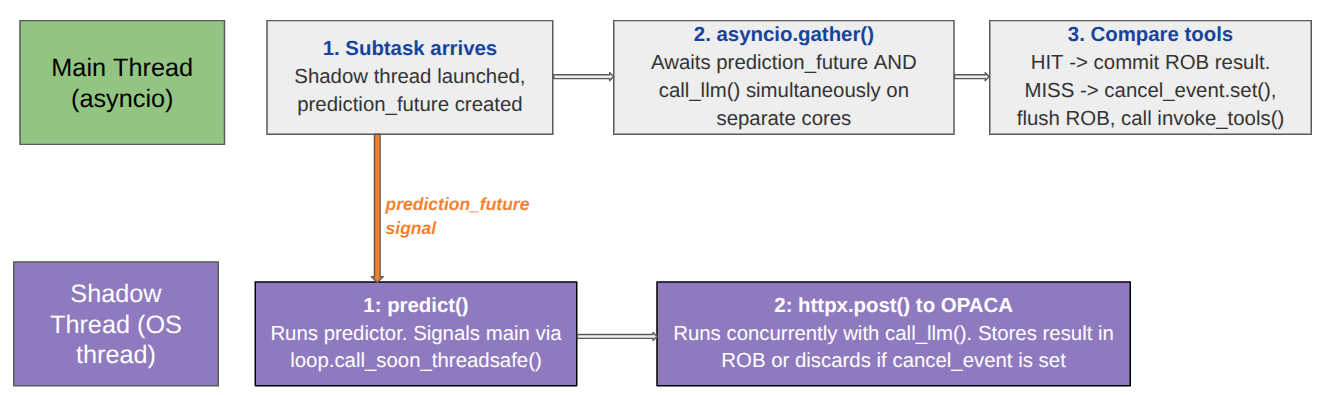
\includegraphics[width=\linewidth]{figures/fig_coordination.png}
  \caption{Asyncio--thread coordination via \texttt{prediction\_future}.
    On subtask arrival the shadow thread is launched and
    \texttt{asyncio.gather()} awaits the prediction future and the main
    LLM call simultaneously on separate cores.
    A HIT commits the ROB; a MISS sets \texttt{cancel\_event} and falls
    back to \texttt{invoke\_tools()}.}
  \label{fig:coordination}
\end{figure}

% ============================================================
\section{Results and Discussion}
% ============================================================

\subsection{Timing Analysis and Speculative Window}
Because the speculative mechanism targets only the tool-execution phase of the orchestration pipeline, the potential latency savings are inherently bounded.
Within the parameters of the current benchmark, a perfect predictor yields a reduction of approximately \textbf{76.7\,ms} for simple queries and
\textbf{228.8\,ms} for complex queries, representing \textbf{2.47\%} and \textbf{3.24\%} of the critical path, respectively, as shown in Figure~\ref{fig:critpath_final}.
While these gains are modest, they establish a definitive upper bound for assessing predictor efficacy and confirm that speculation can recover a reliable portion of execution time without architectural re-engineering.

\begin{figure}[!htbp]
  \centering
  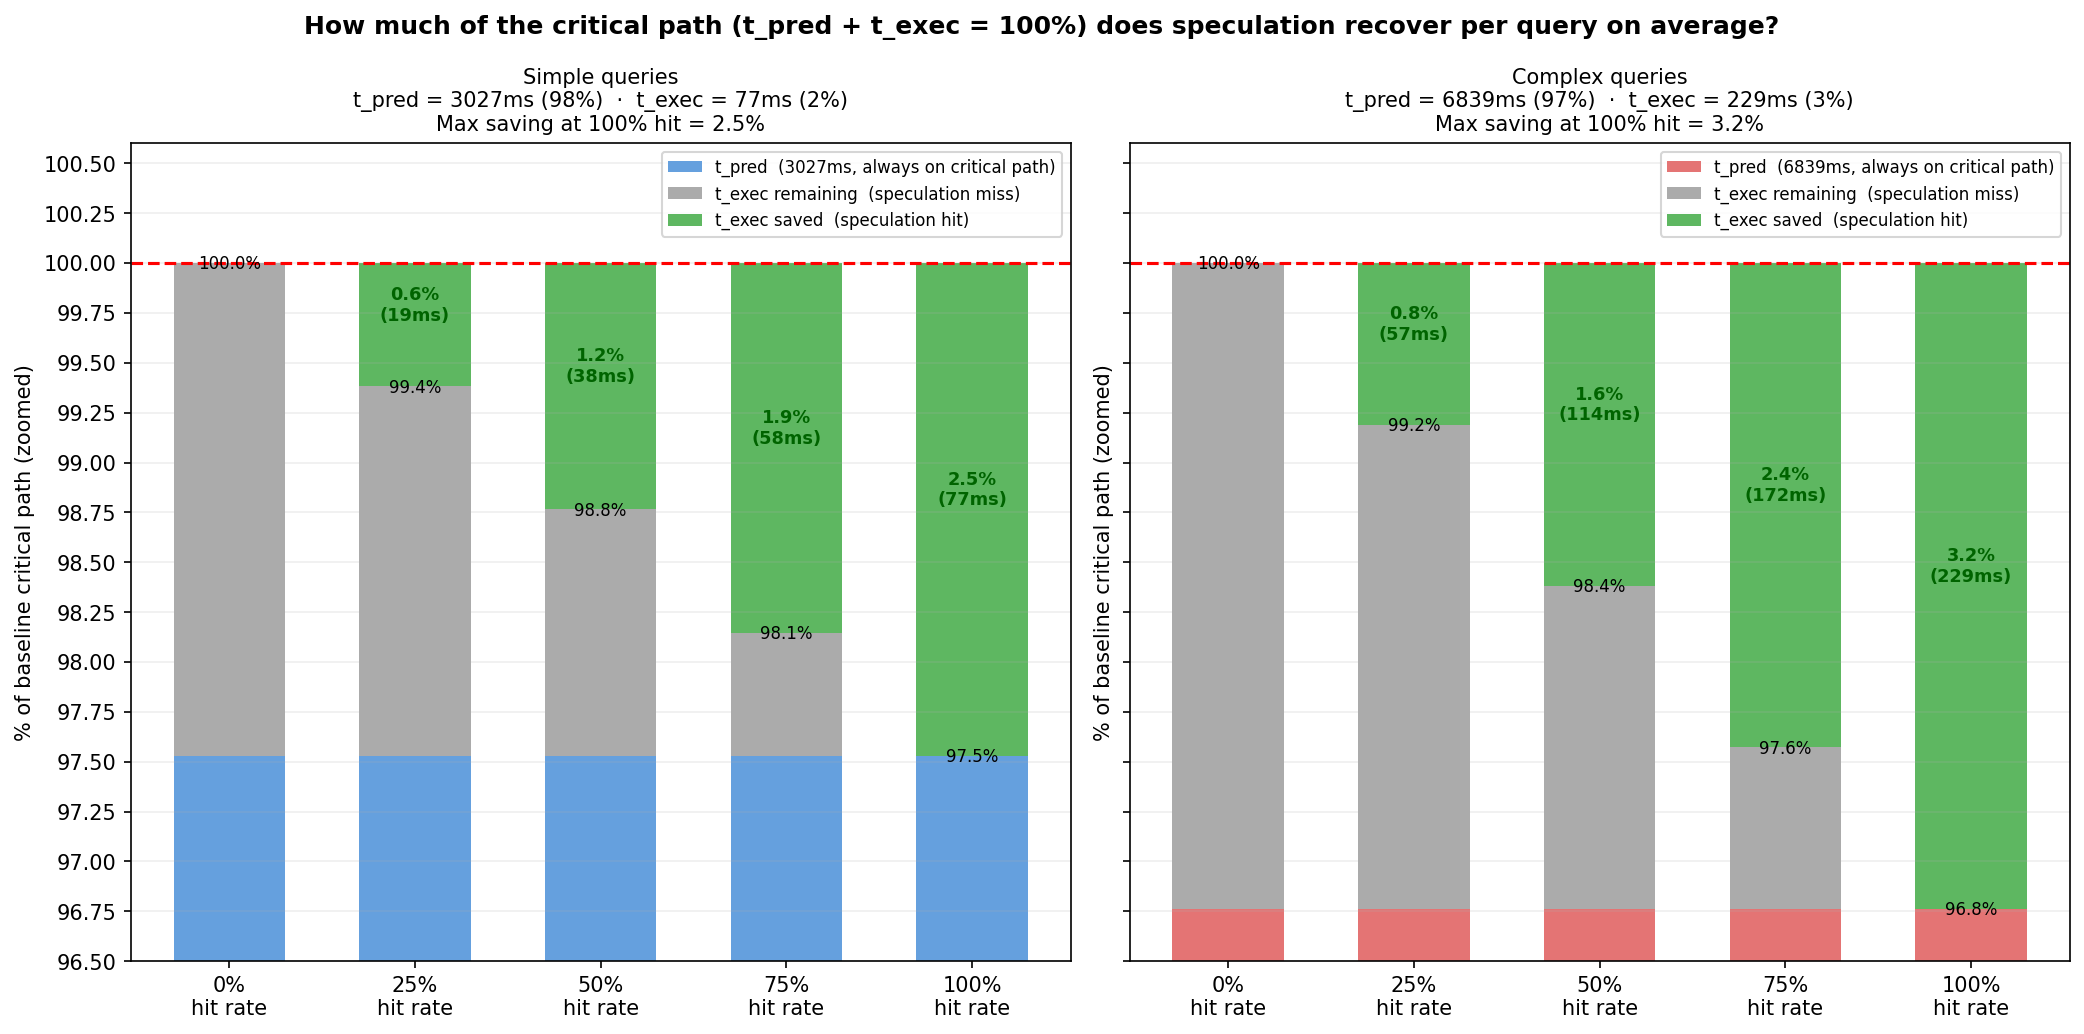
\includegraphics[width=\linewidth]{figures/fig_critpath_final.png}
  \caption{Critical path recovery at hit rates 0--100\%.
    Left: simple queries ($\twtp{=}3027$\,ms, $\twte{=}77$\,ms,
    max saving $\approx 2.47\%$).
    Right: complex queries ($\twtp{=}6839$\,ms, $\twte{=}229$\,ms,
    max saving $\approx 3.24\%$).
    Every value is recoverable at zero cost on a miss.}
  \label{fig:critpath_final}
\end{figure}

The timing profile also confirms that predictor speed is never the limiting factor.
In the context of simple queries the baseline tool-selection phase accounts for
approximately 3027\,ms whereas tool execution requires only 76.7\,ms; a
predictor that runs $5\times$ slower than the baseline still completes with
thousands of milliseconds to spare, as shown in Figure~\ref{fig:5x}.
A similar margin holds for complex queries (6839\,ms vs.\ 228.8\,ms).
The challenge for SAGE++ is therefore not speed but predictive accuracy.

\begin{figure}[!htbp]
  \centering
  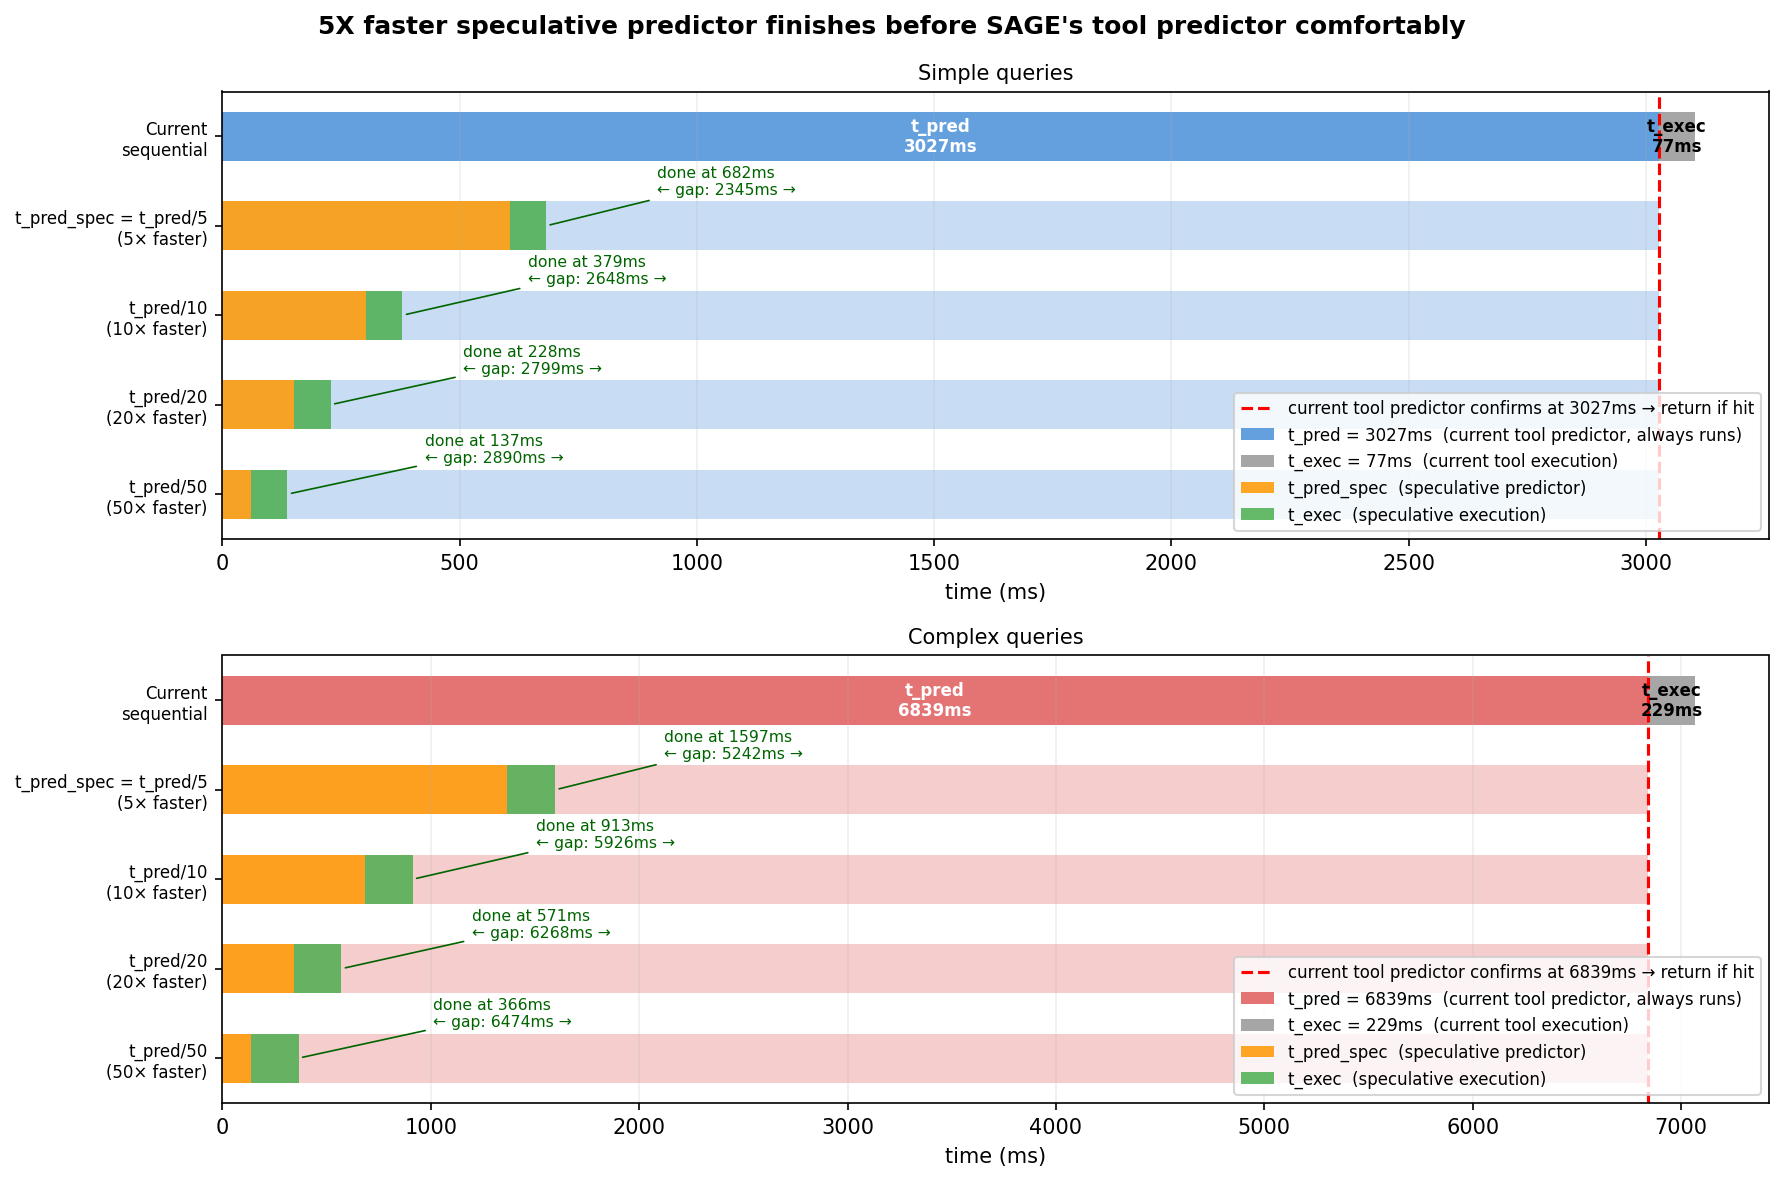
\includegraphics[width=\linewidth]{figures/fig2_5x.png}
  \caption{A speculative predictor $5\times$ slower than SAGE's Worker Tool
    Predictor still finishes with thousands of milliseconds to spare on every
    query. Predictor overhead is never a binding constraint.}
  \label{fig:5x}
\end{figure}

Because the SAGE benchmark uses simulated services without real-world actuation
overhead, $\twte$ in production deployments where tool calls interact with physical sensors, warehouse systems, or database transactions over a network would be substantially larger.
The savings ceiling scales directly with $\twte$, so production deployments are
expected to show proportionally larger absolute savings.

\subsection{Predictor Accuracy}
Figure~\ref{fig:accuracy} reports full tool-sequence accuracy for all four
predictor configurations across simple and complex query types.

\begin{figure}[!htbp]
  \centering
  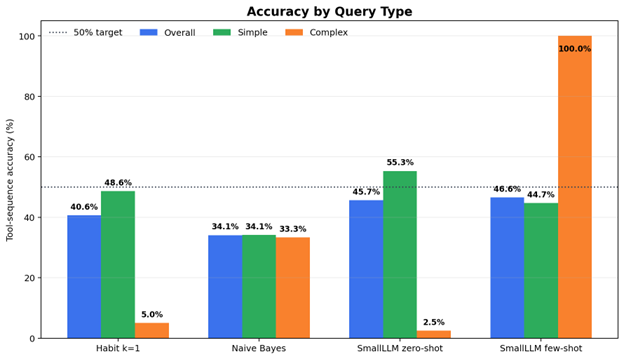
\includegraphics[width=\linewidth]{figures/fig_accuracy.png}
  \caption{Accuracy by query type across all four predictor configurations.
    The dashed line marks the 50\% target.
    SmallLLM few-shot reaches 100\% on complex queries (held-out $n{=}3$;
    interpret with caution).}
  \label{fig:accuracy}
\end{figure}

The Habit predictor ($k{=}1$) achieves \textbf{40.6\%} overall accuracy
(48.6\% simple, 5.0\% complex).
Strong simple-query performance stems from task clustering: the predictor's
compatible-tool fallback handles repeated room-name or availability queries even
when exact signatures differ.
The sharp drop on complex queries reflects the limits of short-range ordering
locality when sequences are longer and repetition is rare.

The Na\"{i}ve Bayes predictor achieves 95.4\% accuracy on the training split.
On the 88-prompt held-out set it maintains a \textbf{34.1\%} overall accuracy (34.1\% simple, 33.3\% complex), demonstrating consistent generalization across query types without the sharp degradation seen in the Habit predictor.

The SmallLLM zero-shot variant achieves \textbf{45.7\%} overall accuracy, peaking at \textbf{55.3\%} on simple prompts but falling to 2.5\% on complex.
The few-shot variant reaches a held-out accuracy of \textbf{46.6\%} overall
(44.7\% simple, \textbf{100.0\%} complex).
The complex-query result must be interpreted with caution: it is based on only three held-out examples and broader validation on an expanded complex dataset is required before drawing strong conclusions.
The broader trend nonetheless substantiates the viability of predictor-guided speculation and positions the few-shot SmallLLM as the most compelling direction for future development.

\subsection{Predictor Speed}
Figure~\ref{fig:speed} compares mean runtime per tool-selection decision across all predictor configurations and the baseline SAGE OpenAI path.

\begin{figure}[!htbp]
  \centering
  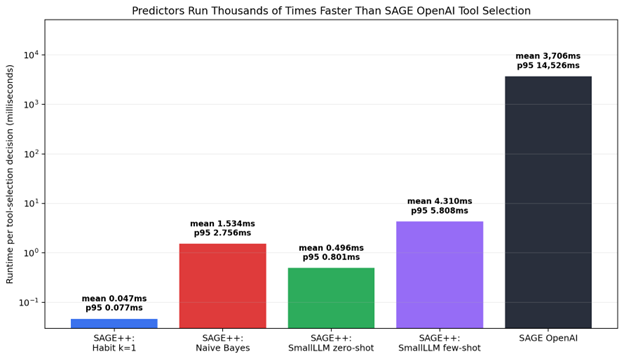
\includegraphics[width=\linewidth]{figures/fig_predictor_speed.png}
  \caption{Runtime per tool-selection decision (log scale).
    All SAGE++ predictors operate orders of magnitude faster than the baseline SAGE OpenAI tool-selection path
    (mean 3706\,ms, p95 14\,526\,ms).}
  \label{fig:speed}
\end{figure}

The Habit predictor is the most lightweight at a mean of \textbf{0.047\,ms}
(p95 0.077\,ms).
Na\"{i}ve Bayes averages \textbf{1.53\,ms} (p95 2.76\,ms), and the zero-shot
SmallLLM averages \textbf{0.50\,ms} (p95 0.80\,ms).
The few-shot SmallLLM is the slowest of the speculative set at
\textbf{4.31\,ms} mean (p95 5.81\,ms), yet remains orders of magnitude faster
than the baseline SAGE OpenAI tool-selection path, which averages
\textbf{3706\,ms} (p95 14\,526\,ms).
These measurements confirm that all implemented predictors satisfy the speed
requirement by a very wide margin, shifting the primary challenge from runtime
to predictive accuracy.

\subsection{Expected Time Savings}
Table~\ref{tab:savings} projects per-query time savings by combining held-out
predictor accuracy with the upper bounds of 76.7\,ms (simple) and 228.8\,ms
(complex) established from the timing analysis:
\begin{equation}
  \mathbb{E}[\text{saving}] = \text{accuracy} \times \twte
\end{equation}

\begin{table}[!htbp]
\centering
\caption{SAGE++ time savings per query.
  (*) complex result from held-out $n{=}3$; interpret with caution.}
\label{tab:savings}
\renewcommand{\arraystretch}{1.3}
\resizebox{\columnwidth}{!}{%
\begin{tabular}{l c c c c}
\toprule
\rowcolor{navy}
\color{white}\textbf{Predictor}
  & \color{white}\textbf{Simple acc.}
  & \color{white}\textbf{Simple savings}
  & \color{white}\textbf{Complex acc.}
  & \color{white}\textbf{Complex savings} \\
\midrule
SmallLLM few-shot  & 44.7\% & $\approx$34.3\,ms & 100.0\%* & $\approx$228.8\,ms* \\
\rowcolor{rowgray}
SmallLLM zero-shot & 55.3\% & $\approx$42.4\,ms & 2.5\%    & $\approx$5.7\,ms \\
Habit $k{=}1$      & 48.6\% & $\approx$37.3\,ms & 5.0\%    & $\approx$11.4\,ms \\
\rowcolor{rowgray}
Na\"{i}ve Bayes    & 34.1\% & $\approx$26.1\,ms & 33.3\%   & $\approx$76.2\,ms \\
\bottomrule
\end{tabular}}
\end{table}

SmallLLM zero-shot recovers the most time on simple queries ($\approx$42.4\,ms)
due to its highest simple-query accuracy.
Na\"{i}ve Bayes provides the most consistent cross-type baseline at
$\approx$26.1\,ms (simple) and $\approx$76.2\,ms (complex).
SmallLLM few-shot represents the most significant research trajectory,
potentially reclaiming the entire 228.8\,ms execution window for complex queries,
though broader validation remains necessary.
All gains are achieved with negligible operational overhead, confirming that
SAGE++ successfully converts predictor-guided speculation into quantifiable
performance enhancements.

% ============================================================
\section{Future Work}
% ============================================================
Future research should prioritize enhancing both predictive accuracy and the
operational scope of the SAGE++ architecture.
The most immediate priority is expanding the benchmark dataset with a more robust
set of complex held-out instances; the current evaluation's skew toward simple
prompts limits the ability to draw definitive conclusions about multi-tool
sequence recovery, and a balanced dataset is essential to verify whether the
few-shot SmallLLM performance holds at scale.

More specialized local LLM predictors while potentially slower than the current lightweight baselines, may still operate comfortably within the expansive execution window provided by the WorkerAgent's decision phase and warrant investigation.

Regarding system safety, the Hazard Detection Unit's blanket restriction on stateful operations is conservative.
Future iterations could explore transactional APIs or compensation mechanisms to enable safe rollback of speculative writes, expanding the set of tools that
benefit from speculation.

The practical value of SAGE++ is expected to be most in domains where $\twte$ is substantial, robotics, financial systems, and real-world actuation environments where external operations dominate the critical path.
Finally, testing the Habit predictor with authentic user interaction traces remains a key objective, as its reliance on short-range ordering locality is expected to yield higher dividends in personalized, repetitive environments than
in standardized benchmark streams.

\begin{thebibliography}{00}
\bibitem{ye2025speculative} N. Ye, A. Ahuja, G. Liargkovas, Y. Lu, K. Kaffes,
  and T. Peng, ``Speculative Actions: A Lossless Framework for Faster Agentic
  Systems,'' \textit{arXiv preprint arXiv:2510.04371}, 2025.
\bibitem{guan2025dsp} Y. Guan, Q. Lan, S. Fei, D. Ding, D. Acharya, C. Wang,
  and W. Hua, ``Dynamic Speculative Agent Planning,''
  \textit{arXiv preprint arXiv:2509.01920}, 2025.
\bibitem{gim2024asynclm} I. Gim, S. S. Lee, and L. Zhong, ``Asynchronous LLM
  Function Calling,'' \textit{arXiv preprint arXiv:2412.07017}, 2024.
\bibitem{huang2025spagent} Z. Huang, W. Zeng, T. Fu, T. Liu, Y. Sun, K. Hong,
  and Y. Wang, ``Reducing Latency of LLM Search Agent via Speculation-Based
  Algorithm-System Co-Design,''
  \textit{arXiv preprint arXiv:2511.20048}, 2025.
\bibitem{xiao2025m1parallel} Y. Xiao \textit{et al.},
  ``M1-Parallel: Parallel Multi-Agent Scheduling,'' 2025.
\bibitem{zhang2025apc} Q. Zhang, M. Wornow, G. Wan, and K. Olukotun,
  ``Agentic Plan Caching: Test-Time Memory for Fast and Cost-Efficient LLM
  Agents,'' \textit{arXiv preprint arXiv:2506.14852}, 2025.
\bibitem{saha2025system1x} S. Saha, A. Prasad, J. C. Y. Chen, P. Hase,
  E. Stengel-Eskin, and M. Bansal, ``System-1.x: Learning to Balance Fast
  and Slow Planning with Language Models,''
  \textit{arXiv preprint arXiv:2407.14414}, 2024.
\bibitem{zhang2025swiftspec} Z. Zhang, Z. Jiang, C. Jiang, M. Yu, S. Zheng,
  H. Lin, H. Hoffmann, and X. Liu,
  ``SwiftSpec: Ultra-Low Latency LLM Decoding by Scaling Asynchronous
  Speculative Decoding,''
  \textit{arXiv preprint arXiv:2506.11309}, 2025.
\bibitem{drammeh2025multiagent} P. Drammeh,
  ``Multi-Agent LLM Orchestration Achieves Deterministic, High-Quality
  Decision Support for Incident Response,''
  \textit{arXiv preprint arXiv:2511.15755}, 2025.
\bibitem{strehlow2026sage} R. K. Strehlow, T. K\"{u}ster, O. F. Kupke,
  B. L. Kurps, F. Sivrikaya, and S. Albayrak,
  ``SAGE: Tool-Augmented LLM Task Solving Strategies in Scalable
  Multi-Agent Environments,''
  \textit{arXiv preprint arXiv:2601.09750}, 2026.
\bibitem{leviathan2023speculative} Y. Leviathan, M. Kalman, and Y. Matias,
  ``Fast Inference from Transformers via Speculative Decoding,''
  \textit{arXiv preprint arXiv:2211.17192}, 2023.
\bibitem{cai2024medusa} T. Cai, Y. Li, Z. Geng, H. Peng, J. D. Lee, D. Chen,
  and T. Dao, ``Medusa: Simple LLM Inference Acceleration Framework with
  Multiple Decoding Heads,''
  \textit{arXiv preprint arXiv:2401.10774}, 2024.
\bibitem{python314freethreading} Python Software Foundation,
  ``Free-threaded CPython,'' \textit{Python 3.14 Documentation}, 2025.
  [Online]. Available:
  \url{https://docs.python.org/3.14/howto/free-threading-python.html}
\end{thebibliography}

\vspace{12pt}
\end{document}